\documentclass[paper=letter,11pt]{scrartcl}

\KOMAoptions{headinclude=true, footinclude=false}
\KOMAoptions{DIV=14, BCOR=5mm}
\KOMAoptions{numbers=noendperiod}
\KOMAoptions{parskip=half}
\addtokomafont{disposition}{\rmfamily}
\addtokomafont{part}{\LARGE}
\addtokomafont{descriptionlabel}{\rmfamily}
%\setkomafont{pageheadfoot}{\normalsize\sffamily}
\setkomafont{pagehead}{\normalsize\rmfamily}
%\setkomafont{publishers}{\normalsize\rmfamily}
\setkomafont{caption}{\normalfont\small}
\setcapindent{0pt}
\deffootnote[1em]{1em}{1em}{\textsuperscript{\thefootnotemark}\ }


\usepackage{amsmath}
\usepackage[varg]{txfonts}
\usepackage[T1]{fontenc}
\usepackage{graphicx}
\usepackage{xcolor}
\usepackage[american]{babel}
% hyperref is needed in many places, so include it here
\usepackage{hyperref}

\usepackage{xspace}
\usepackage{multirow}
\usepackage{float}


\usepackage{braket}
\usepackage{bbm}
\usepackage{relsize}
\usepackage{tcolorbox}


\def\x{\ensuremath{x}}
\def\xp{\ensuremath{x'}}
\def\t{\ensuremath{t}}
\def\tp{\ensuremath{t'}}
\def\v{\ensuremath{v}}
%\def\nus{$\nu$s}

%\def\ketY{\ensuremath{\ket {\Psi}}}
%\def\iGeV{\ensuremath{\textrm{GeV}^{-1}}}
%%\def\mp{\ensuremath{m_{\textrm{proton}}}}
%\def\rp{\ensuremath{r_{\textrm{proton}}}}
%\def\me{\ensuremath{m_{\textrm{electron}}}}
%\def\aG{\ensuremath{\alpha_G}}
%\def\rAtom{\ensuremath{r_{\textrm{atom}}}}
%\def\rNucl{\ensuremath{r_{\textrm{nucleus}}}}
%\def\GN{\ensuremath{\textrm{G}_\textrm{N}}}
%\def\ketX{\ensuremath{\ket{\vec{x}}}}
%\def\ve{\ensuremath{\vec{\epsilon}}}
%
%
%\def\ABCDMatrix{\ensuremath{\begin{pmatrix} A &  B  \\ C  & D \end{pmatrix}}}
%\def\xyprime{\ensuremath{\begin{pmatrix} x' \\ y' \end{pmatrix}}}
%\def\xyprimeT{\ensuremath{\begin{pmatrix} x' &  y' \end{pmatrix}}}
%\def\xy{\ensuremath{\begin{pmatrix} x \\ y \end{pmatrix}}}
%\def\xyT{\ensuremath{\begin{pmatrix} x & y \end{pmatrix}}}
%
%\def\IMatrix{\ensuremath{\begin{pmatrix} 0 &  1  \\ -1  & 0 \end{pmatrix}}}
%\def\IBoostMatrix{\ensuremath{\begin{pmatrix} 0 &  1  \\ 1  & 0 \end{pmatrix}}}
%\def\JThree{\ensuremath{\begin{pmatrix}    0 & -i & 0  \\ i & 0  & 0 \\ 0 & 0 & 0 \end{pmatrix}}} 
%\def\JTwo{\ensuremath{\begin{bmatrix}    0 & 0 & -i  \\ 0 & 0  & 0 \\ i & 0 & 0 \end{bmatrix}}}
%\def\JOne{\ensuremath{\begin{bmatrix}    0 & 0 & 0  \\ 0 & 0  & -i \\ 0 & i & 0 \end{bmatrix}}}
%\def\etamn{\ensuremath{\eta_{\mu\nu}}}
%\def\Lmn{\ensuremath{\Lambda^\mu_\nu}}
%\def\dmn{\ensuremath{\delta^\mu_\nu}}
%\def\wmn{\ensuremath{\omega^\mu_\nu}}
%\def\be{\begin{equation*}}
%\def\ee{\end{equation*}}
%\def\bea{\begin{eqnarray*}}
%\def\eea{\end{eqnarray*}}
%\def\bi{\begin{itemize}}
%\def\ei{\end{itemize}}
%\def\fmn{\ensuremath{F_{\mu\nu}}}
%\def\fMN{\ensuremath{F^{\mu\nu}}}
%\def\bc{\begin{center}}
%\def\ec{\end{center}}
%\def\nus{$\nu$s}

\def\adagger{\ensuremath{a_{p\sigma}^\dagger}}
\def\lineacross{\noindent\rule{\textwidth}{1pt}}

\newcommand{\multiline}[1] {
\begin{tabular} {|l}
#1
\end{tabular}
}

\newcommand{\multilineNoLine}[1] {
\begin{tabular} {l}
#1
\end{tabular}
}



\newcommand{\lineTwo}[2] {
\begin{tabular} {|l}
#1 \\
#2
\end{tabular}
}

\newcommand{\rmt}[1] {
\textrm{#1}
}


%
% Units
%
\def\m{\ensuremath{\rmt{m}}}
\def\GeV{\ensuremath{\rmt{GeV}}}
\def\pt{\ensuremath{p_\rmt{T}}}


\def\parity{\ensuremath{\mathcal{P}}}

\usepackage{cancel}
\usepackage{ mathrsfs }
\def\bigL{\ensuremath{\mathscr{L}}}

\usepackage{ dsfont }

\def\nus{$\nu$s}
\def\nue{\ensuremath{\nu_e}}
\def\numu{\ensuremath{\nu_\mu}}
\def\nutau{\ensuremath{\nu_\tau}}
\def\nualpha{\ensuremath{\nu_\alpha}}
\def\nuone{\ensuremath{\nu_1}}
\def\nutwo{\ensuremath{\nu_2}}
\def\nuthree{\ensuremath{\nu_3}}


\usepackage{fancyhdr}
\fancyhf{}



\lhead{\Large 33-211} % \hfill Introduction to Particle Physics \hfill Spring 2022}
\chead{\Large Physics 3 : Modern Essentials} % \hfill Spring 2022}
\rhead{\Large Spring 2023} % \hfill Introduction to Particle Physics \hfill Spring 2022}
\begin{document}
\thispagestyle{fancy}


\begin{center}
{\huge \textbf{Exam \#3}}
\large

\end{center}

{\large



\textbf{1) Compton Scattering. }\hfill \textit{3 Points}\\
In Compton scattering of X-rays from electrons the outgoing X-rays have shorter wavelength than the incoming X-rays: True or False.

\vspace*{0.4in}

\textbf{2) Bug fixing the Periodic Table. }\hfill \textit{6 Points}\\
Before Moseley, the periodic table was ordered by atomic mass. Mosley showed that it should be ordered by atomic charge.  Describe how was he able to measure the charge on the nucleus Z.

\vfill

\textbf{3) The Frank-Hertz Experiment. }\hfill \textit{7 Points}\\
Describe how the quantization of atomic energies can be observed by looking at electron collisions in gas.

\vfill

\clearpage

\textbf{4) Cathode rays}\hfill \textit{10 Points}\\
Describe Thompson's Cathode-ray experiment that discovered the electron.
What did property of electrons did he measure ?
What was surprising about his result ?

\vspace*{3.4in}

\begin{minipage}{\textwidth}
\textbf{5) Development of the Atomic model. }\hfill \textit{10 Points}\\
Describe Rutherford's experiment testing the atomic model.
What was unexpected about his results~?
How did this change our picture of the atom?
\end{minipage}

\clearpage


\textbf{6) Black body radiation}\hfill \textit{12 Points}\\
Sketch the observed radiation distribution (power radiated / unit area) vs wavelength for a blackbody with temperature 6000 K.
Overlay a sketch of the classical prediction.

\begin{center}
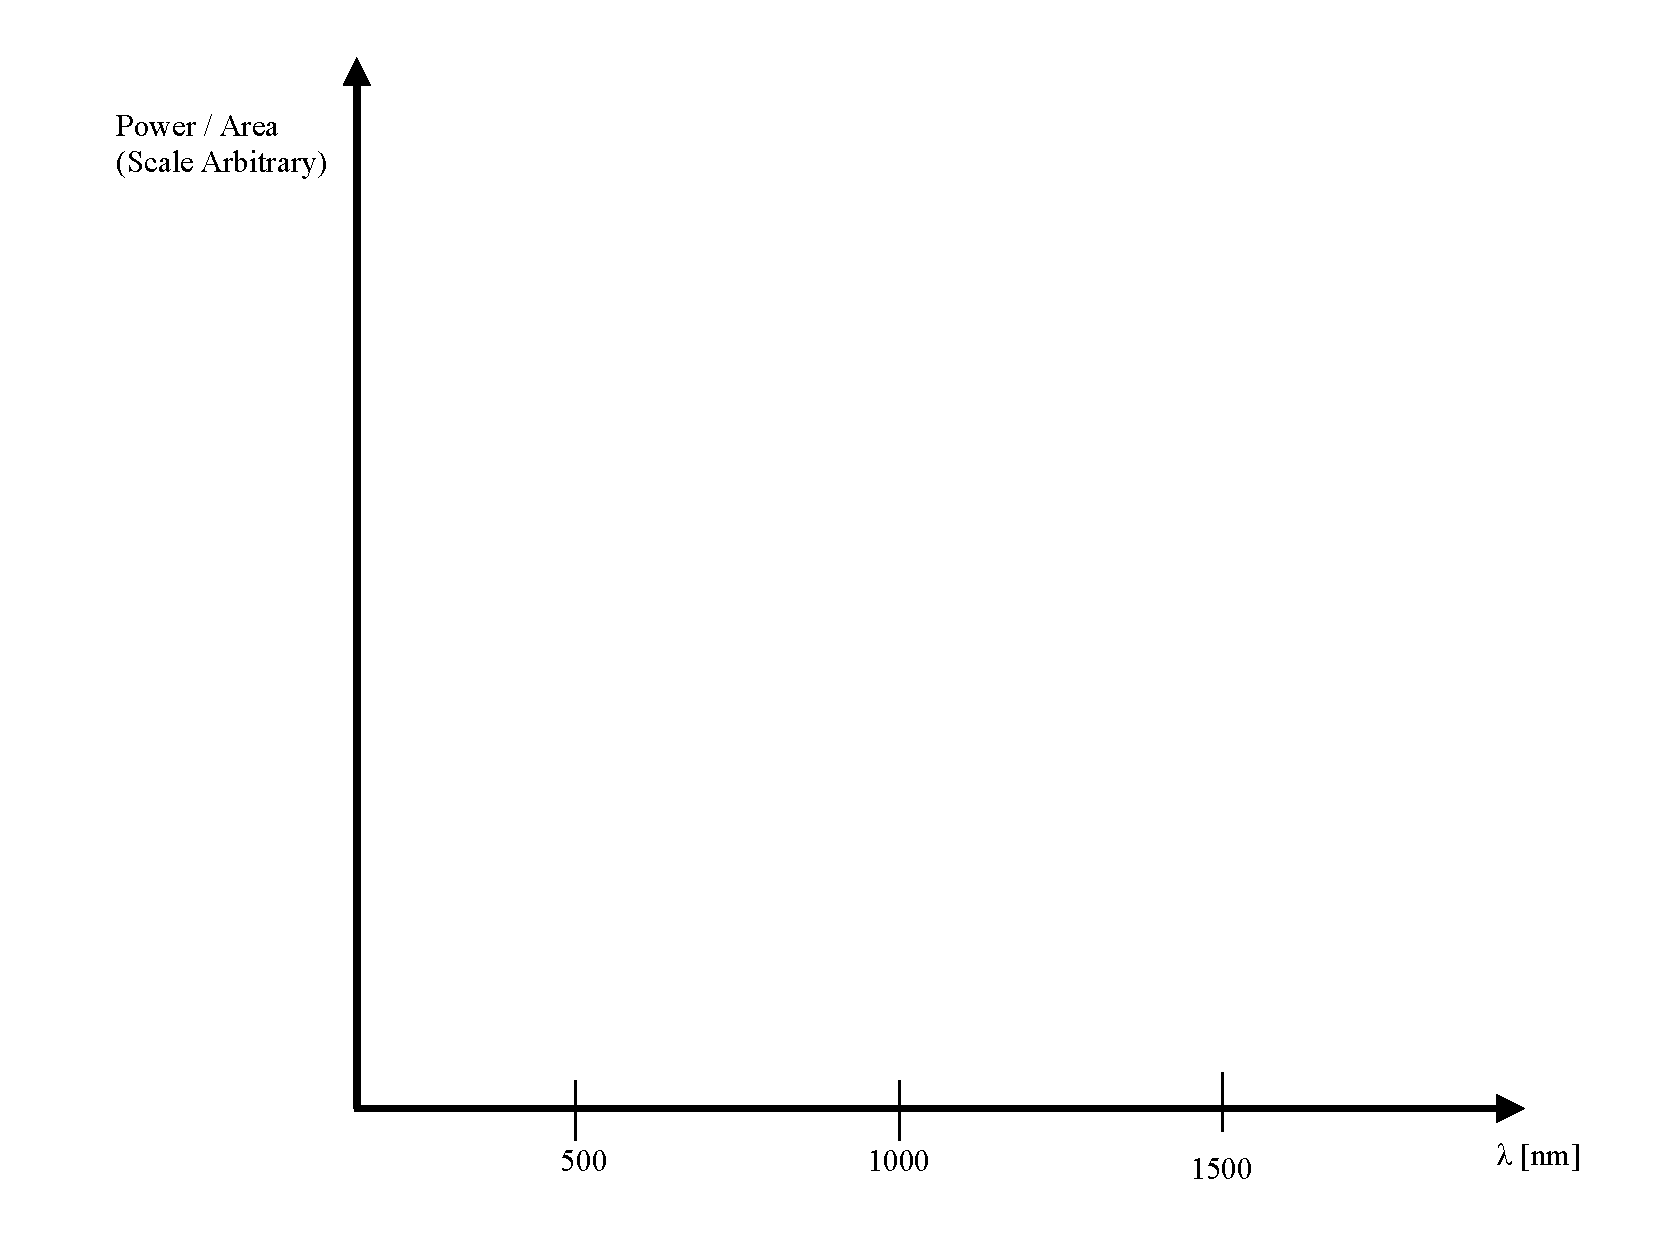
\includegraphics[width=0.65\textwidth]{./Axes.pdf}
\end{center}

In natural units, temperature has units \GeV.  What are the units of power/area in \GeV ? How does the total power output by a star (which is a blackbody) scale with temperature ?

\vspace{1.25in}

\begin{minipage}{\textwidth}
\textbf{7) The Bohr Model of an Atom. }\hfill \textit{7 Points}\\
How was Bohr's model different from the planetary model of atoms that came before it ?
What problems did the Bohr model address ?
\end{minipage}

\vspace{3.25in}


\clearpage

\textbf{8) Photoelectric Effect }\hfill \textit{(10 points)}\\

Suppose we are shinning a beam of ultraviolet light of known wavelength onto a metal surface with a binding energy of electrons (or work function) is 2.0 eV

\begin{itemize}
\item[a)] If this light liberates photo-electrons of maximum kinetic energy 3.0 eV, what is the wavelength of the light?
\vfill
\item[b)] Suppose the intensity of the light impinging upon the metal surface is tripled. What do you expect to happen to the number of electrons liberated from the surface? Explain.
\vfill
\item[c)] Suppose instead that the wavelength of the light is tripled. What do you expect to happen to the number of electrons liberated from the surface? Explain.
\vfill
\end{itemize}

\clearpage

\textbf{9) Particles As Waves } \hfill \textit{15 Points}
\begin{itemize}
\item[a)] Use the uncertainty principle to estimate the energy of an electron in an infinite square well of width L.
\vspace*{2.5in}
\item[b)] Use the uncertainty principle to estimate the size of a hydrogen atom (V = -$\alpha/r$). \\ \textit{(Express your result in terms of $m_e$. $\alpha$ )}
          Do you need to worry about relativistic effects when analyzing the Hydrogen atom ?  Justify your answer.
\vspace*{2.5in}
\item[c)] Use the uncertainty principle to estimate the size of a muonium atom. Muonium is the bound state of a muon (m=0.1 \GeV) and a proton.
          Do you need to worry about relativistic effects when analyzing Muonium  ?  Justify your answer. 
%\vspace*{2.in}
\end{itemize}



} % Begning Large
\end{document}
